% Options for packages loaded elsewhere
\PassOptionsToPackage{unicode}{hyperref}
\PassOptionsToPackage{hyphens}{url}

%
\documentclass[
]{article}
\usepackage{amsmath,amssymb}
\usepackage{iftex}
\ifPDFTeX
  \usepackage[T1]{fontenc}
  \usepackage[utf8]{inputenc}
  \usepackage{textcomp} % provide euro and other symbols
\else % if luatex or xetex
  \usepackage{unicode-math} % this also loads fontspec
  \defaultfontfeatures{Scale=MatchLowercase}
  \defaultfontfeatures[\rmfamily]{Ligatures=TeX,Scale=1}
\fi
\usepackage{lmodern}
\ifPDFTeX\else
  % xetex/luatex font selection
\fi
% Use upquote if available, for straight quotes in verbatim environments
\IfFileExists{upquote.sty}{\usepackage{upquote}}{}
\IfFileExists{microtype.sty}{% use microtype if available
  \usepackage[]{microtype}
  \UseMicrotypeSet[protrusion]{basicmath} % disable protrusion for tt fonts
}{}
\makeatletter
\@ifundefined{KOMAClassName}{% if non-KOMA class
  \IfFileExists{parskip.sty}{%
    \usepackage{parskip}
  }{% else
    \setlength{\parindent}{0pt}
    \setlength{\parskip}{6pt plus 2pt minus 1pt}}
}{% if KOMA class
  \KOMAoptions{parskip=half}}
\makeatother
\usepackage{xcolor}
\usepackage{color}
\usepackage{fancyvrb}
\newcommand{\VerbBar}{|}
\newcommand{\VERB}{\Verb[commandchars=\\\{\}]}
\DefineVerbatimEnvironment{Highlighting}{Verbatim}{commandchars=\\\{\}}
% Add ',fontsize=\small' for more characters per line
\newenvironment{Shaded}{}{}
\newcommand{\AlertTok}[1]{\textcolor[rgb]{1.00,0.00,0.00}{\textbf{#1}}}
\newcommand{\AnnotationTok}[1]{\textcolor[rgb]{0.38,0.63,0.69}{\textbf{\textit{#1}}}}
\newcommand{\AttributeTok}[1]{\textcolor[rgb]{0.49,0.56,0.16}{#1}}
\newcommand{\BaseNTok}[1]{\textcolor[rgb]{0.25,0.63,0.44}{#1}}
\newcommand{\BuiltInTok}[1]{\textcolor[rgb]{0.00,0.50,0.00}{#1}}
\newcommand{\CharTok}[1]{\textcolor[rgb]{0.25,0.44,0.63}{#1}}
\newcommand{\CommentTok}[1]{\textcolor[rgb]{0.38,0.63,0.69}{\textit{#1}}}
\newcommand{\CommentVarTok}[1]{\textcolor[rgb]{0.38,0.63,0.69}{\textbf{\textit{#1}}}}
\newcommand{\ConstantTok}[1]{\textcolor[rgb]{0.53,0.00,0.00}{#1}}
\newcommand{\ControlFlowTok}[1]{\textcolor[rgb]{0.00,0.44,0.13}{\textbf{#1}}}
\newcommand{\DataTypeTok}[1]{\textcolor[rgb]{0.56,0.13,0.00}{#1}}
\newcommand{\DecValTok}[1]{\textcolor[rgb]{0.25,0.63,0.44}{#1}}
\newcommand{\DocumentationTok}[1]{\textcolor[rgb]{0.73,0.13,0.13}{\textit{#1}}}
\newcommand{\ErrorTok}[1]{\textcolor[rgb]{1.00,0.00,0.00}{\textbf{#1}}}
\newcommand{\ExtensionTok}[1]{#1}
\newcommand{\FloatTok}[1]{\textcolor[rgb]{0.25,0.63,0.44}{#1}}
\newcommand{\FunctionTok}[1]{\textcolor[rgb]{0.02,0.16,0.49}{#1}}
\newcommand{\ImportTok}[1]{\textcolor[rgb]{0.00,0.50,0.00}{\textbf{#1}}}
\newcommand{\InformationTok}[1]{\textcolor[rgb]{0.38,0.63,0.69}{\textbf{\textit{#1}}}}
\newcommand{\KeywordTok}[1]{\textcolor[rgb]{0.00,0.44,0.13}{\textbf{#1}}}
\newcommand{\NormalTok}[1]{#1}
\newcommand{\OperatorTok}[1]{\textcolor[rgb]{0.40,0.40,0.40}{#1}}
\newcommand{\OtherTok}[1]{\textcolor[rgb]{0.00,0.44,0.13}{#1}}
\newcommand{\PreprocessorTok}[1]{\textcolor[rgb]{0.74,0.48,0.00}{#1}}
\newcommand{\RegionMarkerTok}[1]{#1}
\newcommand{\SpecialCharTok}[1]{\textcolor[rgb]{0.25,0.44,0.63}{#1}}
\newcommand{\SpecialStringTok}[1]{\textcolor[rgb]{0.73,0.40,0.53}{#1}}
\newcommand{\StringTok}[1]{\textcolor[rgb]{0.25,0.44,0.63}{#1}}
\newcommand{\VariableTok}[1]{\textcolor[rgb]{0.10,0.09,0.49}{#1}}
\newcommand{\VerbatimStringTok}[1]{\textcolor[rgb]{0.25,0.44,0.63}{#1}}
\newcommand{\WarningTok}[1]{\textcolor[rgb]{0.38,0.63,0.69}{\textbf{\textit{#1}}}}
\usepackage{longtable,booktabs,array}
\usepackage{calc} % for calculating minipage widths
% Correct order of tables after \paragraph or \subparagraph
\usepackage{etoolbox}
\makeatletter
\patchcmd\longtable{\par}{\if@noskipsec\mbox{}\fi\par}{}{}
\makeatother
% Allow footnotes in longtable head/foot
\IfFileExists{footnotehyper.sty}{\usepackage{footnotehyper}}{\usepackage{footnote}}
\makesavenoteenv{longtable}
\usepackage{graphicx}
\makeatletter
\def\maxwidth{\ifdim\Gin@nat@width>\linewidth\linewidth\else\Gin@nat@width\fi}
\def\maxheight{\ifdim\Gin@nat@height>\textheight\textheight\else\Gin@nat@height\fi}
\makeatother
% Scale images if necessary, so that they will not overflow the page
% margins by default, and it is still possible to overwrite the defaults
% using explicit options in \includegraphics[width, height, ...]{}
\setkeys{Gin}{width=\maxwidth,height=\maxheight,keepaspectratio}
% Set default figure placement to htbp
\makeatletter
\def\fps@figure{htbp}
\makeatother
\setlength{\emergencystretch}{3em} % prevent overfull lines
\providecommand{\tightlist}{%
  \setlength{\itemsep}{0pt}\setlength{\parskip}{0pt}}
\setcounter{secnumdepth}{-\maxdimen} % remove section numbering
\ifLuaTeX
  \usepackage{selnolig}  % disable illegal ligatures
\fi
\IfFileExists{bookmark.sty}{\usepackage{bookmark}}{\usepackage{hyperref}}
\IfFileExists{xurl.sty}{\usepackage{xurl}}{} % add URL line breaks if available
\urlstyle{same}
\hypersetup{
  hidelinks,
  pdfcreator={LaTeX via pandoc}}

\author{}
\date{}


%-----------------------------------------------------------------------------------
\setlength{\textwidth}{6.9in} \setlength{\textheight}{9.2in}
\hoffset -2.cm \voffset -2.0cm \pagestyle{empty}
%----------------------------------------------------------------------------------
\begin{document}

\hypertarget{1-parameter-estimate-in-coupled-oscillators-system}{%
\section{1 parameter estimate in Coupled-Oscillators
system}\label{1-parameter-estimate-in-coupled-oscillators-system}}

\hypertarget{general-solution}{%
\subsection{General Solution}\label{general-solution}}

The system is given below

\begin{center}
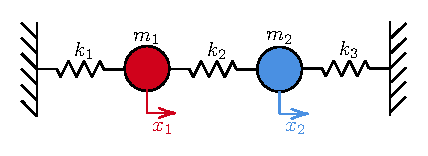
\includegraphics{/Users/yangchangmao/Documents/Coupled-Oscillators/MCMC-note/fig/system.pdf}
\end{center}

denote the \(x_1\) and \(x_2\) are the displacement of two masses
\(m_1\) and \(m_2\) respectively, and \(k_i\) are the springs constant
for \(i=1,2,3\). Also, using \(\vec{x}\) denote two displacement

\[\vec{x} = \begin{pmatrix}x_1\\x_2\end{pmatrix},\]

then the general solution is

\[\vec{x}\left(t\right) = \sum_{i=1}^{2}\left(A_{i}e^{\omega_i t}+ B_{i}e^{-\omega_i t}\right)\vec{\mu}_i,\]

where \(\vec{\mu}_1,\vec{\mu}_2\) are the eigenvector of matrix

\[\mathcal{F} = \begin{pmatrix}
 \displaystyle - \frac{k_1+k_2}{m_1}	&\displaystyle  \frac{k_2}{m_1}\\
 \displaystyle  \frac{k_2}{m_2} 		&\displaystyle  -\frac{k_2+k_3}{m_2}
 \end{pmatrix},\]

\(\lambda_i = \omega_i^2\) for \(i=1,2\) are the eigenvalue of matrix
\(\mathcal{F}\), and \(A_i, B_i\) for \(i=1,2\) are the coefficients
which are given by

\[\begin{pmatrix}A_{1}&B_{1}\\A_{2}&B_{2}\end{pmatrix}
=
\begin{pmatrix}
\hat{\mu}^{-1}\vec{x}\left(0\right) & 
\hat{\omega}^{-1}\hat{\mu}^{-1}\vec{v}\left(0\right)
\end{pmatrix}\begin{pmatrix}1&1\\ 1&-1\end{pmatrix},\]

where

\[\hat{\mu} = \begin{pmatrix}\vec{\mu}_1&\vec{\mu}_2\end{pmatrix}, \quad 
	\hat{\omega} = \begin{pmatrix}\omega_1&0\\0&\omega_2\end{pmatrix},\quad
	\hat{C} = \begin{pmatrix}A_{1}&B_{1}\\A_{2}&B_{2}\end{pmatrix},\]

and

\[\vec{x}\left(0\right) = \begin{pmatrix}x_1\left(0\right)\\x_2\left(0\right)\end{pmatrix}
,\quad
\vec{v}\left(0\right) = \begin{pmatrix}v_1\left(0\right)\\v_2\left(0\right)\end{pmatrix}\]

\newpage

\hypertarget{parameter-estimating}{%
\subsection{Parameter Estimating}\label{parameter-estimating}}

The general solution tells us that after recording the data, this system
have following parameter need be solved.

\begin{longtable}[]{@{}lll@{}}
\toprule\noalign{}
Name & Math notation & Code notation \\
\midrule\noalign{}
\endhead
\bottomrule\noalign{}
\endlastfoot
spring constant & \(k_1, k_2, k_3\) & \texttt{k\ =\ (k1,\ k2,\ k3)} \\
mass & \(m_1, m_2\) & \texttt{m\ =\ (m1,\ m2)} \\
initial position & \(\vec{x}\left(0\right)\) &
\texttt{xi\ =\ (x1i,\ x2i)} \\
initial velocity & \(\vec{v}\left(0\right)\) &
\texttt{vi\ =\ (v1i,\ v2i)} \\
\end{longtable}

\begin{quote}
notice that for the numerical data, we also have a time duration input.

\begin{longtable}[]{@{}lll@{}}
\toprule\noalign{}
Name & Math notation & Code notation \\
\midrule\noalign{}
\endhead
\bottomrule\noalign{}
\endlastfoot
time & \(t = 0\sim t_{\rm end}\) &
\texttt{t\ =\ np.array({[}0,\ ...,\ t\_end{]})} \\
\end{longtable}
\end{quote}

In order to simplify, I choosing \(k_2\) to be the parameter that need
to be estimated by MCMC method.

Fisrt, I crate a target data to be a pseudo experimental data

\begin{Shaded}
\begin{Highlighting}[]
\NormalTok{t }\OperatorTok{=}\NormalTok{ np.arange(}\DecValTok{0}\NormalTok{,}\DecValTok{5}\NormalTok{,}\FloatTok{0.01}\NormalTok{)}
\NormalTok{k }\OperatorTok{=}\NormalTok{ (}\DecValTok{100}\NormalTok{,}\DecValTok{100}\NormalTok{,}\DecValTok{100}\NormalTok{)}
\NormalTok{m }\OperatorTok{=}\NormalTok{ (}\FloatTok{1.0}\NormalTok{, }\FloatTok{1.0}\NormalTok{)}
\NormalTok{xi }\OperatorTok{=}\NormalTok{ (}\FloatTok{0.0}\NormalTok{, }\OperatorTok{{-}}\FloatTok{0.2}\NormalTok{)}
\NormalTok{vi }\OperatorTok{=}\NormalTok{ (}\DecValTok{0}\NormalTok{, }\DecValTok{0}\NormalTok{)}
\NormalTok{(x1\_data, x2\_data, v1\_data, v2\_data) }\OperatorTok{=}\NormalTok{ Model(t, k, m, xi, vi)}
\end{Highlighting}
\end{Shaded}

If we plot \(x_1\) and \(x_2\) verse \(t\) we get the tragetory of two
masses

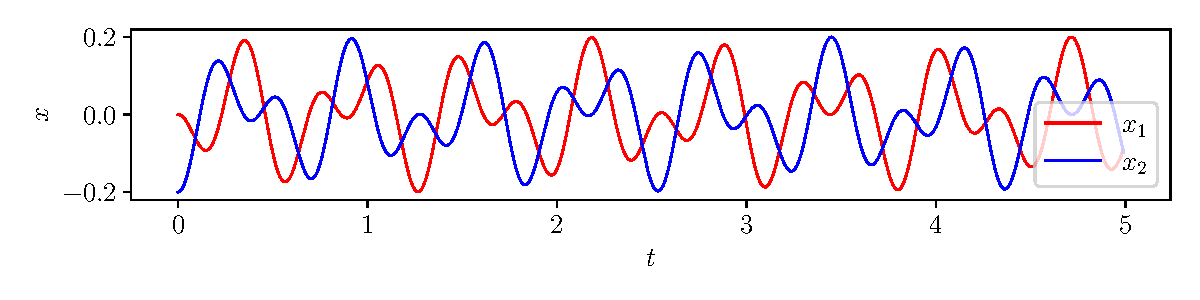
\includegraphics{/Users/yangchangmao/Documents/Coupled-Oscillators/MCMC-note/fig/exp-data.pdf}


\newpage
\hypertarget{mean-square-error}{%
\subsection{Mean Square Error}\label{mean-square-error}}

I define the mean square error (MSE) to be

\[E_{\rm MSE}\left(\vec{k}\right) = \frac{1}{N}\sum_{i=1}^{2}\sum_{j=0}^{N-1}\left(x_{i,j}-x_{\rm theory,j}\left(\vec{k}\right)\right)^2,\]

where the experimental position data points are given by

\[x_{i,j},\quad j=0,1,\ldots, N-1,\]

where \(i=1,2\) denote the two masses position, and
\(\vec{k}=\left(k_1,k_2,k_3\right)\) denote the spring constant.

In implementation, I define a function return MSE

\begin{Shaded}
\begin{Highlighting}[]
\KeywordTok{def}\NormalTok{ MSE(t, k, x1\_data, x2\_data, m, xi, vi):}
\NormalTok{    N }\OperatorTok{=} \BuiltInTok{len}\NormalTok{(t)}
\NormalTok{    x1\_theo, x2\_theo, v1\_theo ,v2\_theo }\OperatorTok{=}\NormalTok{ Model(t, k, m, xi, vi)}
\NormalTok{    MSE1 }\OperatorTok{=}\NormalTok{ np.}\BuiltInTok{sum}\NormalTok{((x1\_data }\OperatorTok{{-}}\NormalTok{ x1\_theo)}\OperatorTok{**}\DecValTok{2}\NormalTok{) }\OperatorTok{/}\NormalTok{ N}
\NormalTok{    MSE2 }\OperatorTok{=}\NormalTok{ np.}\BuiltInTok{sum}\NormalTok{((x2\_data }\OperatorTok{{-}}\NormalTok{ x2\_theo)}\OperatorTok{**}\DecValTok{2}\NormalTok{) }\OperatorTok{/}\NormalTok{ N}
    \ControlFlowTok{return}\NormalTok{ MSE1}\OperatorTok{+}\NormalTok{MSE2}
\end{Highlighting}
\end{Shaded}

\hypertarget{properties-of-mean-square-error}{%
\subsubsection{Properties of Mean Square
Error}\label{properties-of-mean-square-error}}

\begin{quote}
!!! All the properties are calculated while fixing
\texttt{t,\ k1,\ k3,\ m,\ xi,\ vi} and plot for changing \texttt{k2}
\end{quote}

\hypertarget{comparison-parameters}{%
\paragraph{Comparison parameters}\label{comparison-parameters}}

\begin{Shaded}
\begin{Highlighting}[]
\NormalTok{t  }\OperatorTok{=}\NormalTok{ np.arange(}\DecValTok{0}\NormalTok{, }\DecValTok{5}\NormalTok{, }\FloatTok{0.01}\NormalTok{)}
\NormalTok{k1 }\OperatorTok{=} \DecValTok{100}
\NormalTok{k2 }\OperatorTok{=}\NormalTok{ np.arange(}\OperatorTok{{-}}\DecValTok{50}\NormalTok{, }\DecValTok{300}\NormalTok{, }\DecValTok{3000}\NormalTok{)}
\NormalTok{k3 }\OperatorTok{=} \DecValTok{100}
\NormalTok{m  }\OperatorTok{=}\NormalTok{ (}\FloatTok{1.0}\NormalTok{, }\FloatTok{1.0}\NormalTok{)}
\NormalTok{xi }\OperatorTok{=}\NormalTok{ (}\FloatTok{0.0}\NormalTok{, }\OperatorTok{{-}}\FloatTok{0.2}\NormalTok{)}
\NormalTok{vi }\OperatorTok{=}\NormalTok{ (}\DecValTok{0}\NormalTok{, }\DecValTok{0}\NormalTok{)}
\end{Highlighting}
\end{Shaded}

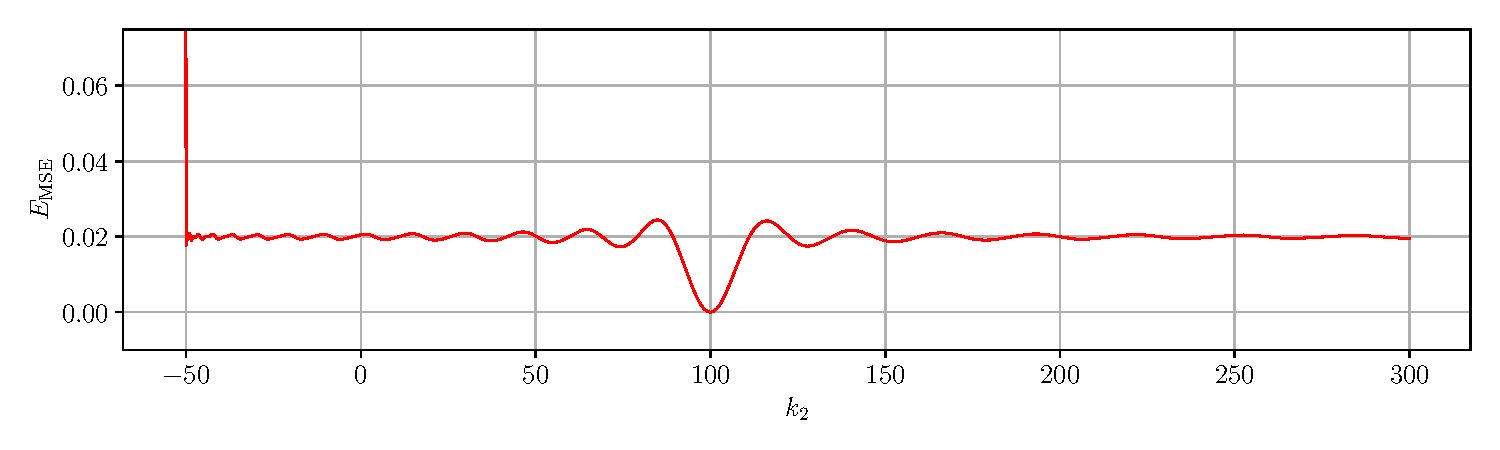
\includegraphics{/Users/yangchangmao/Documents/Coupled-Oscillators/MCMC-note/fig/MSE.pdf}

\begin{itemize}
\item
  MSE has \textbf{global minimum} value at \(k_2 = 100\)
\item
  MSE has many \textbf{local minimum} near target value. For local
  minimum

  \begin{itemize}
  \item
    The value of \(k_2\) farther away from the target, the smaller the
    MSE value is.
  \item
    \textbf{Distance} between every local minimum, start to

    \begin{enumerate}
    \def\labelenumi{\arabic{enumi}.}
    \item
      \textbf{increase} when \(k_2\) bigger than target,
    \item
      \textbf{decrease} when \(k_2\) smaller than target
    \end{enumerate}
  \end{itemize}
\item
  MSE is \textbf{diverge} when value of \(k_2\) is negative.
\item
  MSE is \textbf{oscillation}.
\item
  MSE value is approximate to \(0.02\) for \(k_2>0\)
\end{itemize}

\hypertarget{not-zero-initial-velocity}{%
\paragraph{\texorpdfstring{Not-zero initial velocity
}{Not-zero initial velocity }}\label{not-zero-initial-velocity}}

\begin{Shaded}
\begin{Highlighting}[]
\NormalTok{t  }\OperatorTok{=}\NormalTok{ np.arange(}\DecValTok{0}\NormalTok{, }\DecValTok{5}\NormalTok{, }\FloatTok{0.01}\NormalTok{)}
\NormalTok{k1 }\OperatorTok{=} \DecValTok{100}
\NormalTok{k2 }\OperatorTok{=}\NormalTok{ np.arange(}\OperatorTok{{-}}\DecValTok{50}\NormalTok{, }\DecValTok{300}\NormalTok{, }\DecValTok{3000}\NormalTok{)}
\NormalTok{k3 }\OperatorTok{=} \DecValTok{100}
\NormalTok{m  }\OperatorTok{=}\NormalTok{ (}\FloatTok{1.0}\NormalTok{, }\FloatTok{1.0}\NormalTok{)}
\NormalTok{xi }\OperatorTok{=}\NormalTok{ (}\FloatTok{0.0}\NormalTok{, }\OperatorTok{{-}}\FloatTok{0.2}\NormalTok{)}
\NormalTok{vi }\OperatorTok{=}\NormalTok{ (}\DecValTok{10}\NormalTok{, }\OperatorTok{{-}}\DecValTok{10}\NormalTok{)}
\end{Highlighting}
\end{Shaded}

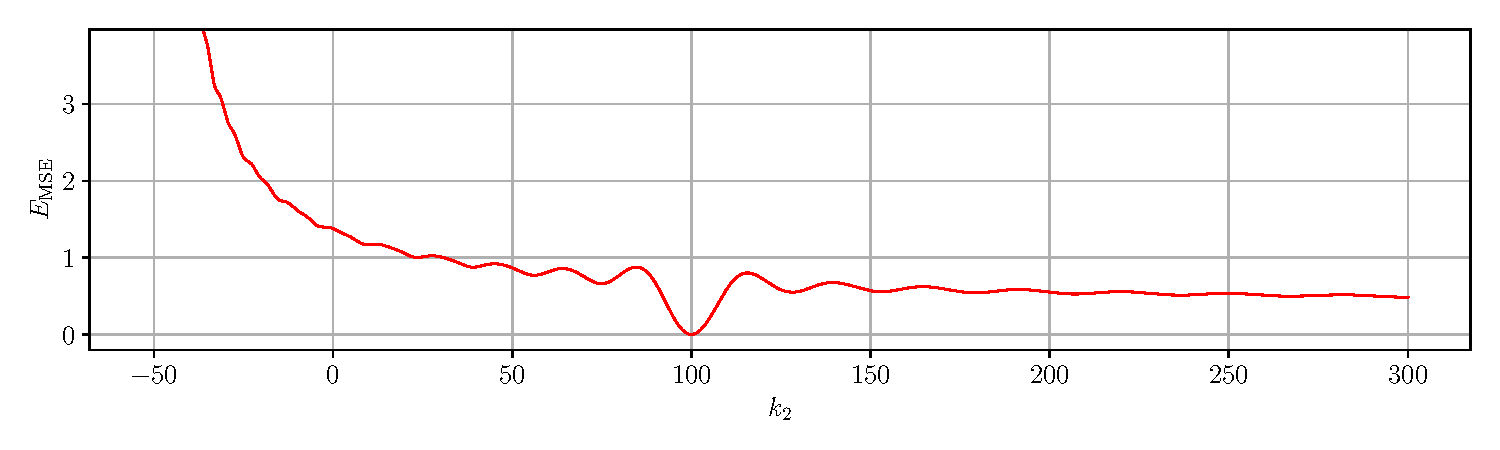
\includegraphics{/Users/yangchangmao/Documents/Coupled-Oscillators/MCMC-note/fig/MSE_v.pdf}

\begin{itemize}
\item
  When initial velocity is not zero, the MSE will increase
  \textbf{exponentially} when \(k_2\) decrease.
\end{itemize}

\hypertarget{bigger-time-duration}{%
\paragraph{Bigger time duration}\label{bigger-time-duration}}

\begin{Shaded}
\begin{Highlighting}[]
\NormalTok{t  }\OperatorTok{=}\NormalTok{ np.arange(}\DecValTok{0}\NormalTok{, }\DecValTok{30}\NormalTok{, }\FloatTok{0.01}\NormalTok{)}
\NormalTok{k1 }\OperatorTok{=} \DecValTok{100}
\NormalTok{k2 }\OperatorTok{=}\NormalTok{ np.arange(}\OperatorTok{{-}}\DecValTok{50}\NormalTok{, }\DecValTok{300}\NormalTok{, }\DecValTok{3000}\NormalTok{)}
\NormalTok{k3 }\OperatorTok{=} \DecValTok{100}
\NormalTok{m  }\OperatorTok{=}\NormalTok{ (}\FloatTok{1.0}\NormalTok{, }\FloatTok{1.0}\NormalTok{)}
\NormalTok{xi }\OperatorTok{=}\NormalTok{ (}\FloatTok{0.0}\NormalTok{, }\OperatorTok{{-}}\FloatTok{0.2}\NormalTok{)}
\NormalTok{vi }\OperatorTok{=}\NormalTok{ (}\DecValTok{0}\NormalTok{, }\DecValTok{0}\NormalTok{)}
\end{Highlighting}
\end{Shaded}

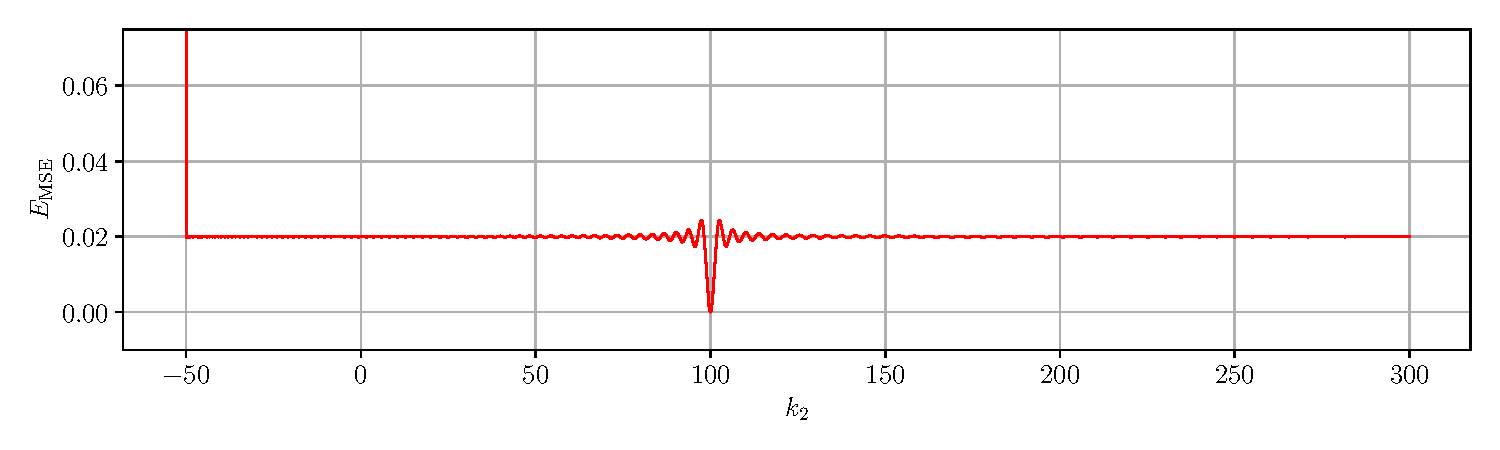
\includegraphics{/Users/yangchangmao/Documents/Coupled-Oscillators/MCMC-note/fig/MSE_t.pdf}

\begin{itemize}
\item
  When we obtain additional experimental data over a longer period of
  time, the oscillation frequency of the MSE value will increase.
\end{itemize}

\hypertarget{shape-of-local-minimum-and-maximum}{%
\paragraph{Shape of Local minimum and
maximum}\label{shape-of-local-minimum-and-maximum}}

Using the same parameters as original setting, and find the local
minimum and maximum of MSE.

\begin{Shaded}
\begin{Highlighting}[]
\NormalTok{t  }\OperatorTok{=}\NormalTok{ np.arange(}\DecValTok{0}\NormalTok{, }\DecValTok{5}\NormalTok{, }\FloatTok{0.01}\NormalTok{)}
\NormalTok{k1 }\OperatorTok{=} \DecValTok{100}
\NormalTok{k2 }\OperatorTok{=}\NormalTok{ np.arange(}\OperatorTok{{-}}\DecValTok{50}\NormalTok{, }\DecValTok{300}\NormalTok{, }\DecValTok{3000}\NormalTok{)}
\NormalTok{k3 }\OperatorTok{=} \DecValTok{100}
\NormalTok{m  }\OperatorTok{=}\NormalTok{ (}\FloatTok{1.0}\NormalTok{, }\FloatTok{1.0}\NormalTok{)}
\NormalTok{xi }\OperatorTok{=}\NormalTok{ (}\FloatTok{0.0}\NormalTok{, }\OperatorTok{{-}}\FloatTok{0.2}\NormalTok{)}
\NormalTok{vi }\OperatorTok{=}\NormalTok{ (}\DecValTok{0}\NormalTok{, }\DecValTok{0}\NormalTok{)}
\end{Highlighting}
\end{Shaded}

Then fitting the local minimum and maximum to get the shape of them

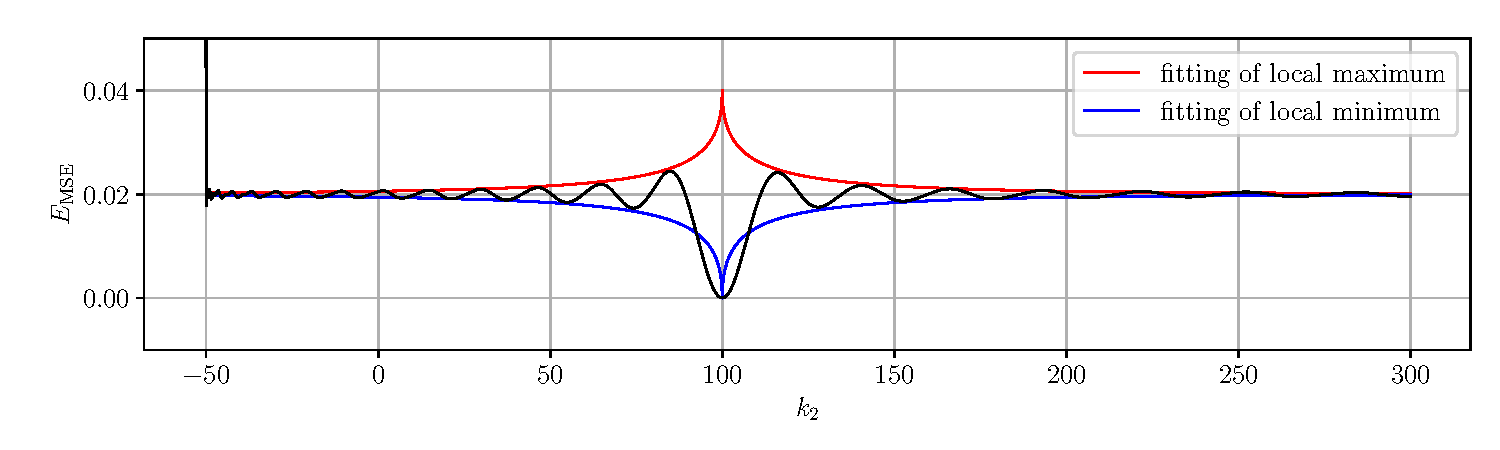
\includegraphics{/Users/yangchangmao/Documents/Coupled-Oscillators/MCMC-note/fig/MSE_peak.pdf}

Result is given by

\[f\left(x\right) = 0.02\left(1\pm e^{-\left(A\left|x-100\right|\right)^{n}}\right)\]

where \(A\approx 0.128373292639\) and \(n\approx 0.496684867617\), that
means the shape of local minimum and maximum are all approximating to
\(e^{-\sqrt{x}}\).

\hypertarget{probability}{%
\subsection{Probability}\label{probability}}

\hypertarget{original-probability}{%
\subsubsection{Original Probability}\label{original-probability}}

If we define the probability to be

\[P\left(\vec{k}\right) = \exp\left(-E_{\rm MSE}\left(\vec{k}\right)\right)\]

Using above data, plot the probability for \(k_2=-50\sim 300\)

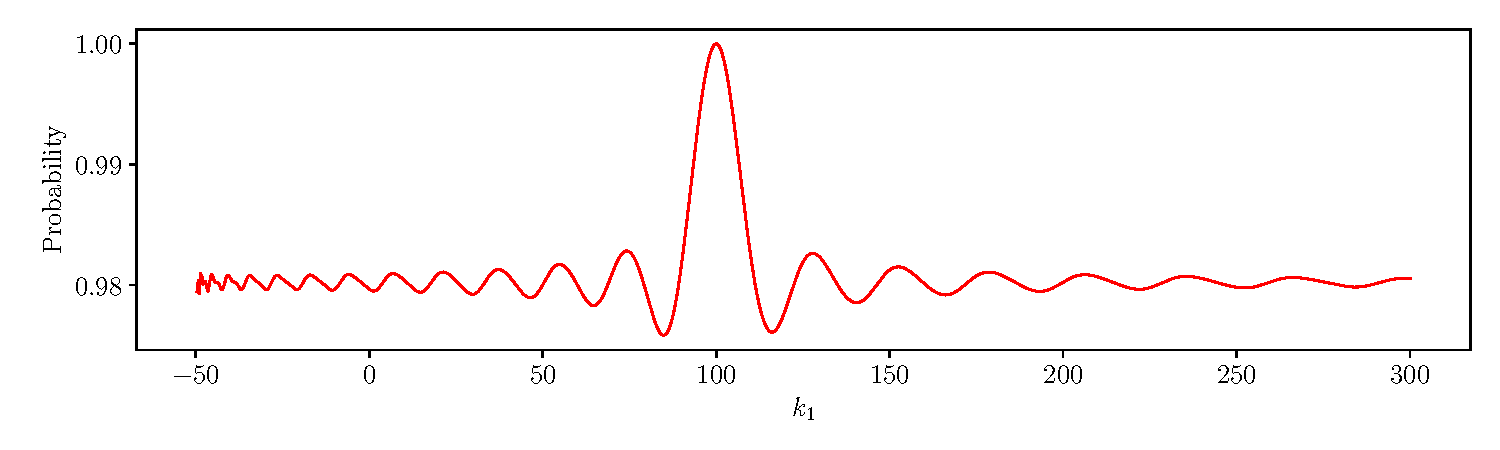
\includegraphics{/Users/yangchangmao/Documents/Coupled-Oscillators/MCMC-note/fig/Prob1.pdf}

\begin{itemize}
\item
  All the value of probability is oscillating near \(0.98\), since
  \(\exp(-0.02)\approx 0.9801\)
\end{itemize}

This may not be favorable for MCMC since I am using this probability to execute MCMC, and the acceptance rate is consistently above 0.8. Therefore, I think I need to modify the shape of the overall probability by decreasing the portions that originally have smaller values.

\hypertarget{transformed-probability}{%
\subsubsection{Transformed Probability}\label{transformed-probability}}

We have known that value of \(E_{\rm MSE}\) is

\[E_{\rm MSE}\in \left[0, \infty\right)\]

and

\[e^{-x} \in \left(0, 1\right], \quad \forall x \left[0, \infty\right)\]

Therefore, if I want to reduce the smaller values, I can employ
\href{https://en.wikipedia.org/wiki/Gamma_correction}{Gamma Correction},
which is commonly used in image processing.

The value of original probability is from \(0\) to \(1\). I defined a
transform function \(T\) as

\[T\left(x\right)=x^{\gamma}\]

and choosing \(\gamma=500\). Now, Using above data, plot the probability
for \(k_2=-50\sim 300\)

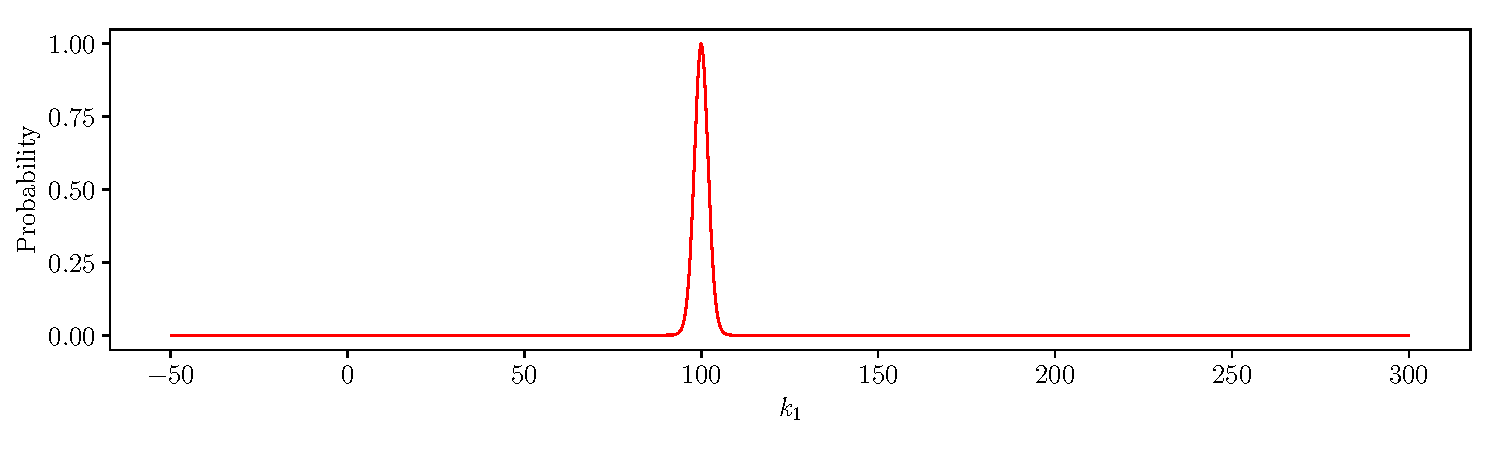
\includegraphics{/Users/yangchangmao/Documents/Coupled-Oscillators/MCMC-note/fig/Prob2.pdf}

This prabability is very close to normal distribution, I think it is
easily good for searching its peak by MCMC method.


\newpage
\hypertarget{mcmc-result}{%
\subsection{MCMC result}\label{mcmc-result}}

Acceptance rate : \(0.15840\)

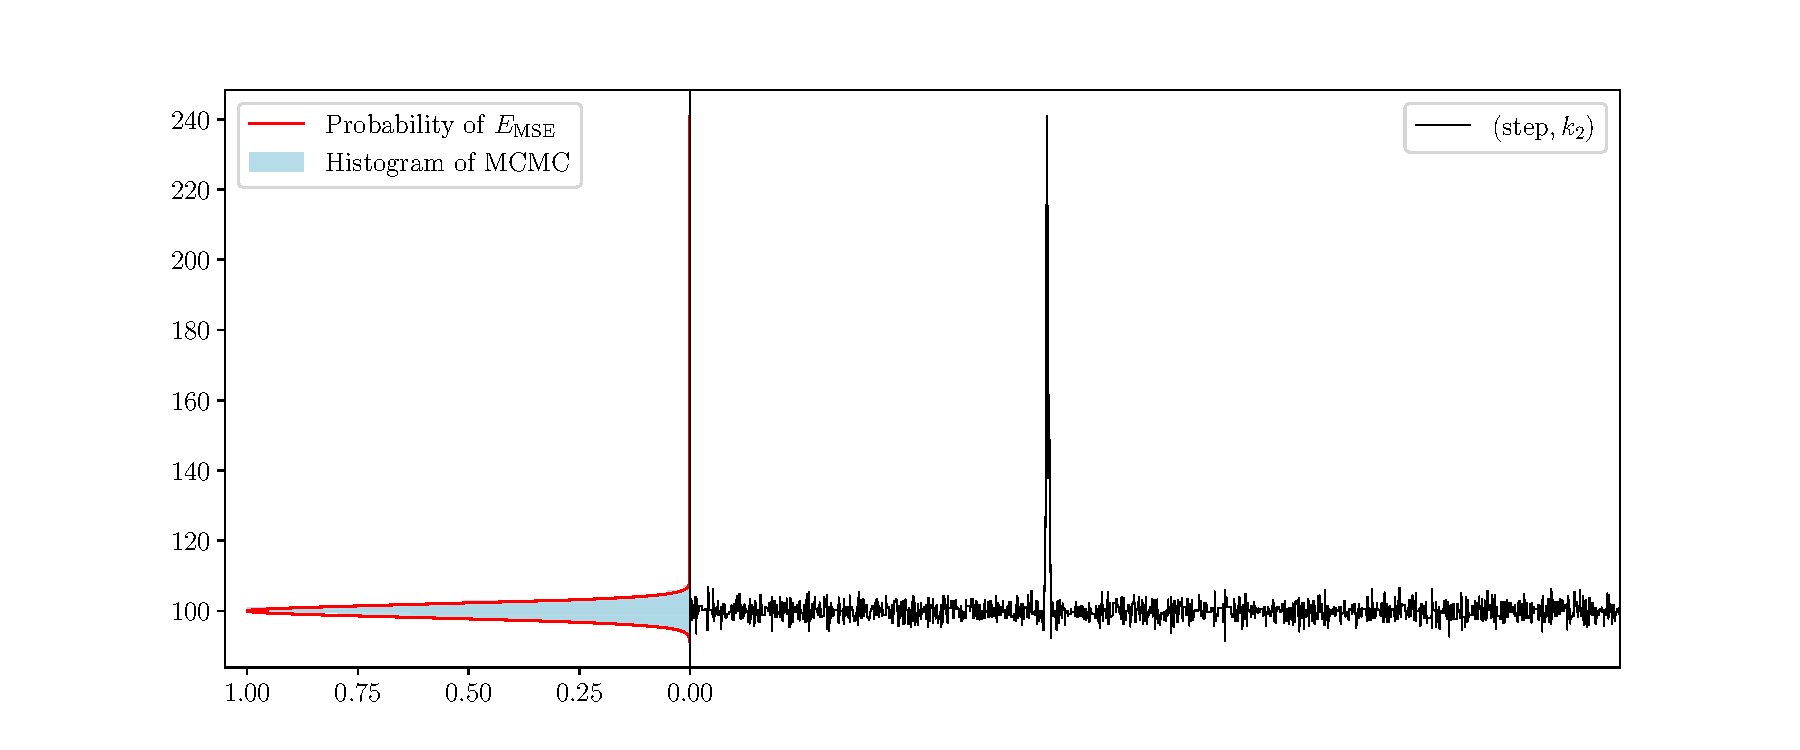
\includegraphics{/Users/yangchangmao/Documents/Coupled-Oscillators/MCMC-note/fig/MCMC-acc0.15840.pdf}

Acceptance rate : \(0.20710\)

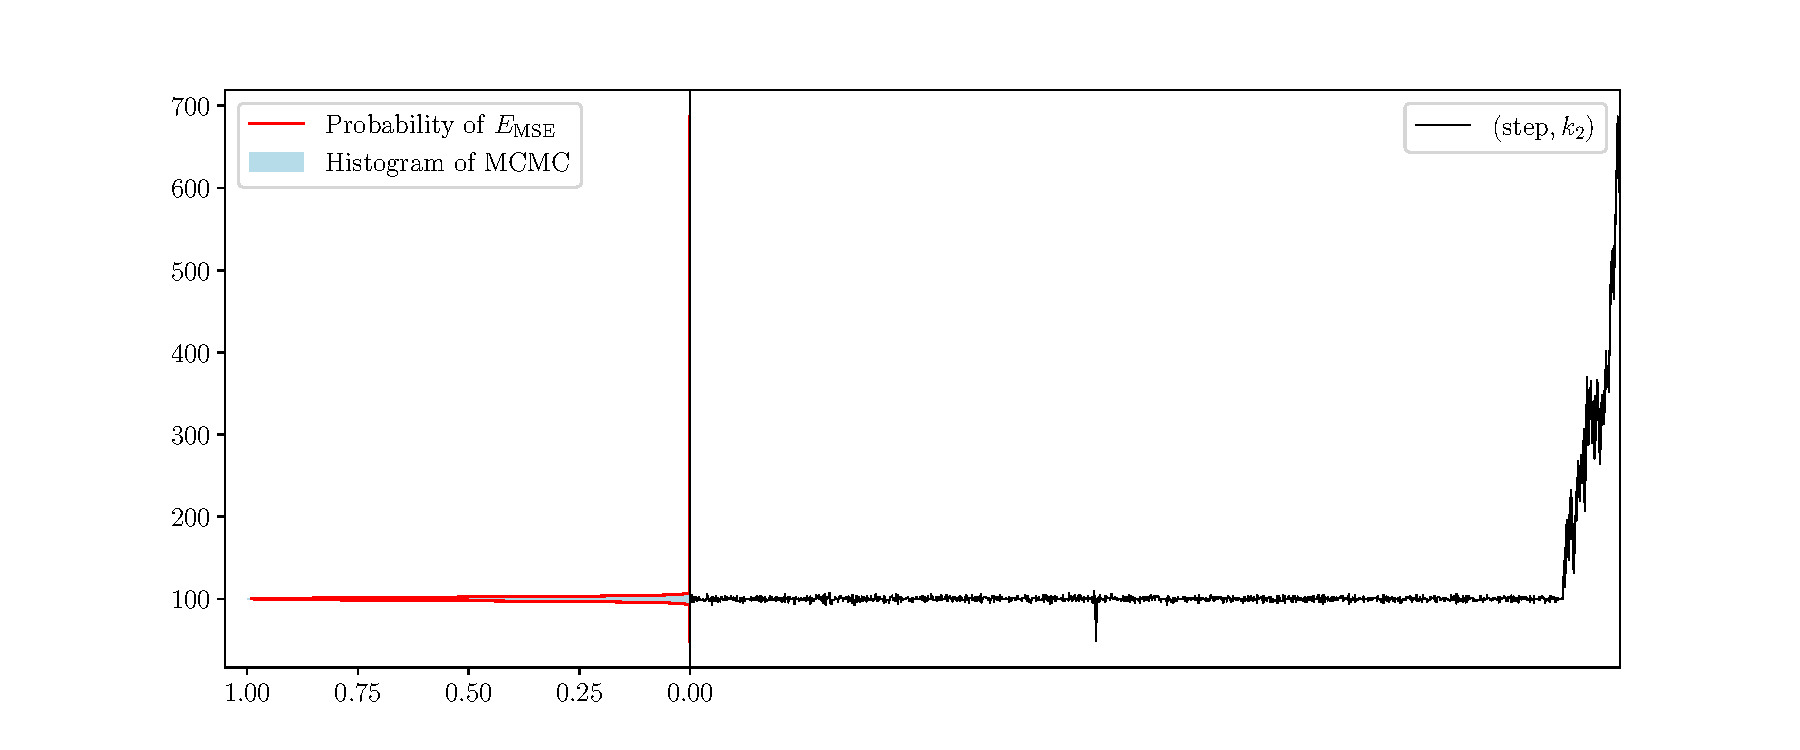
\includegraphics{/Users/yangchangmao/Documents/Coupled-Oscillators/MCMC-note/fig/MCMC-acc0.20710.pdf }

Acceptance rate : \(0.30980\)

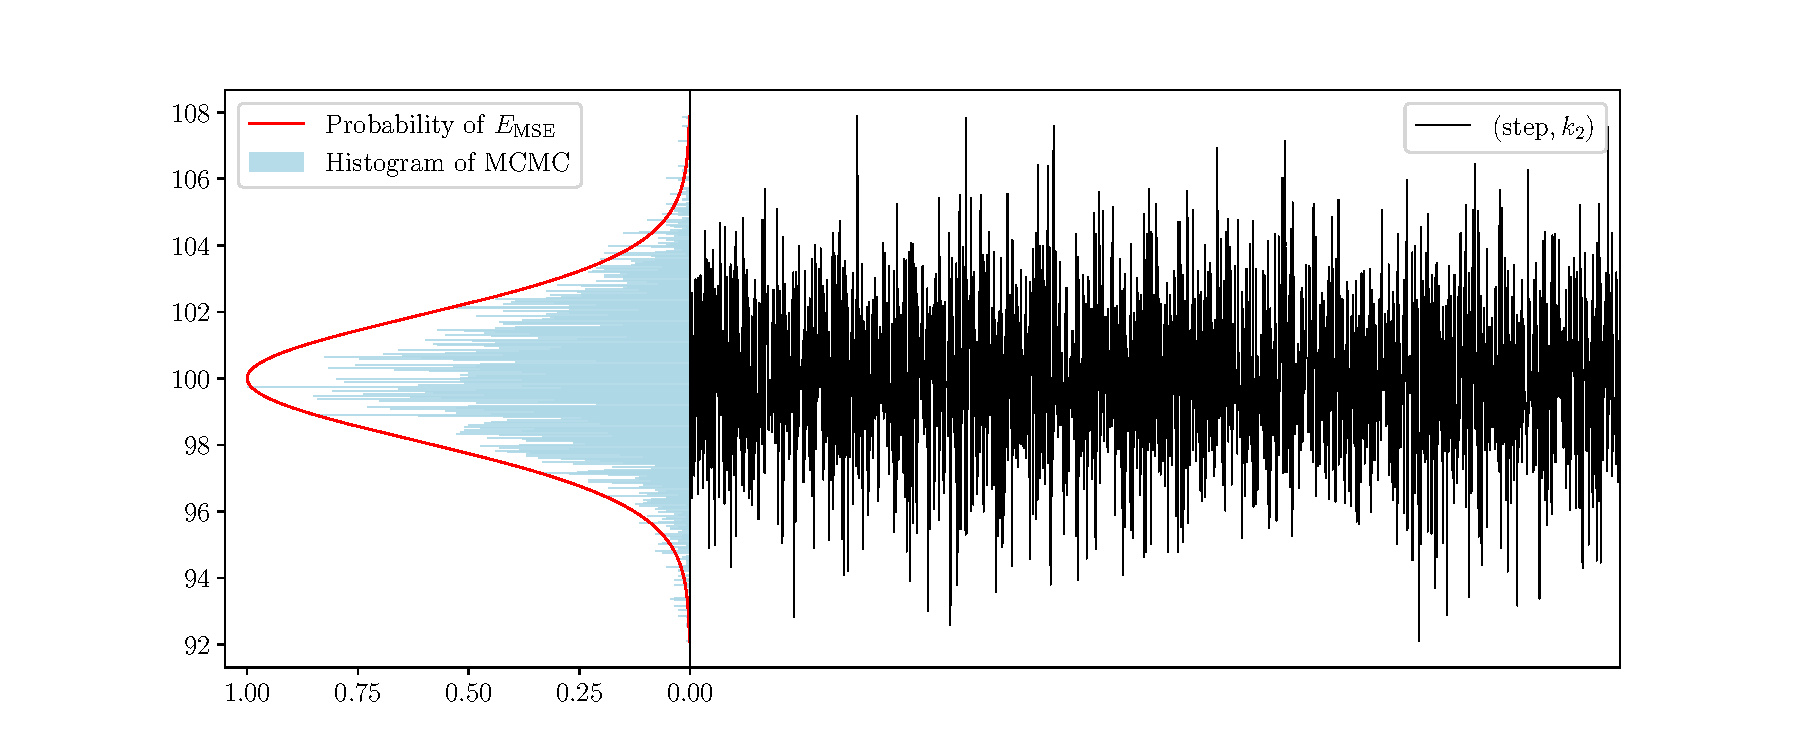
\includegraphics{/Users/yangchangmao/Documents/Coupled-Oscillators/MCMC-note/fig/MCMC-acc0.30980.pdf}

Acceptance rate : \(0.16320\)

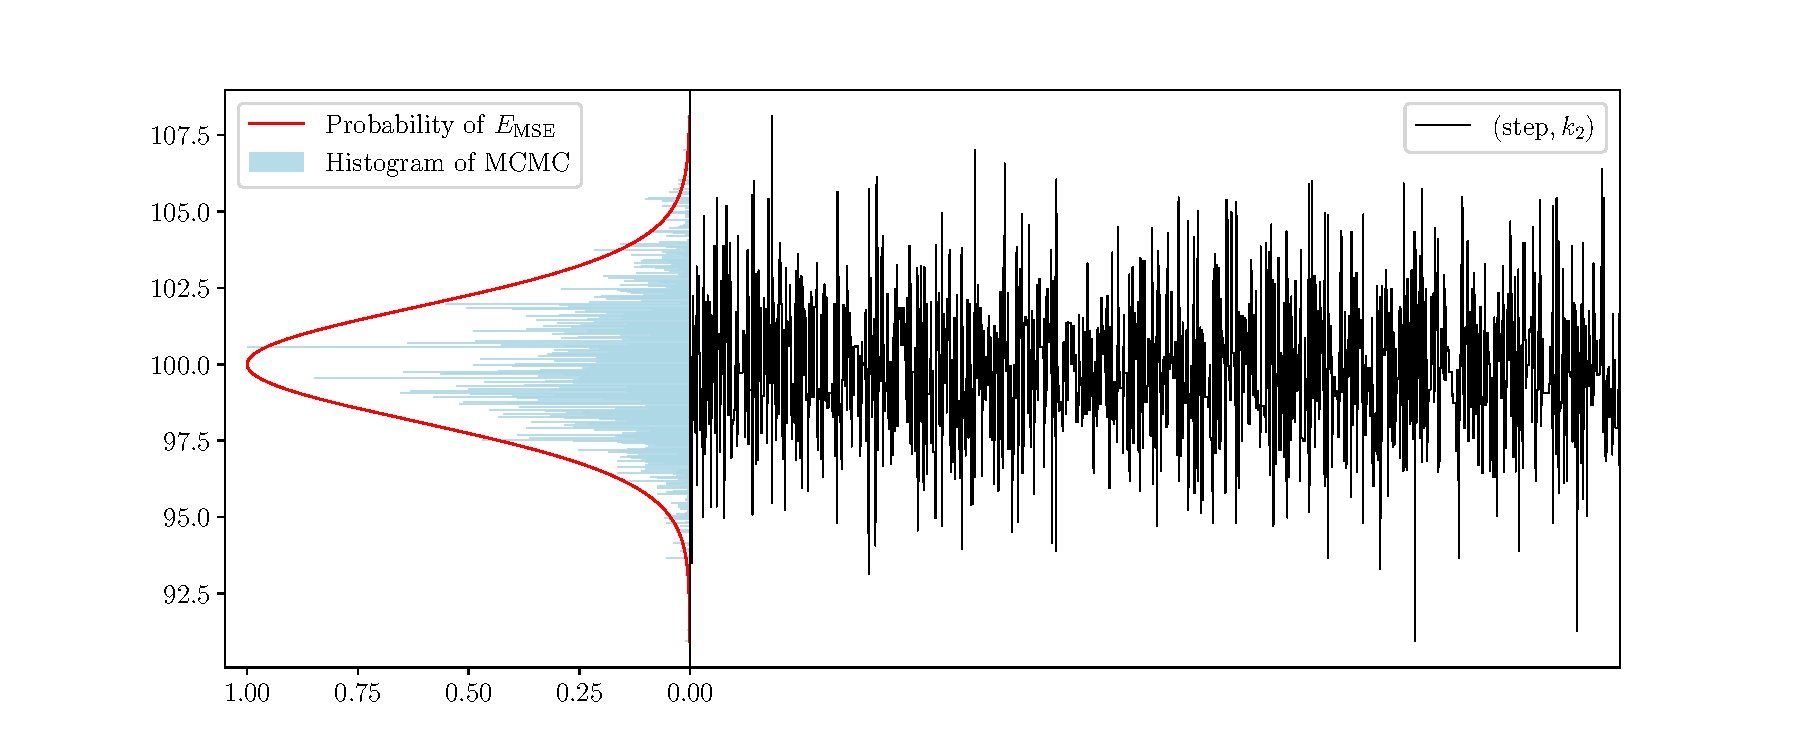
\includegraphics{/Users/yangchangmao/Documents/Coupled-Oscillators/MCMC-note/fig/MCMC-acc0.16320.pdf }

Acceptance rate : \(0.22080\)

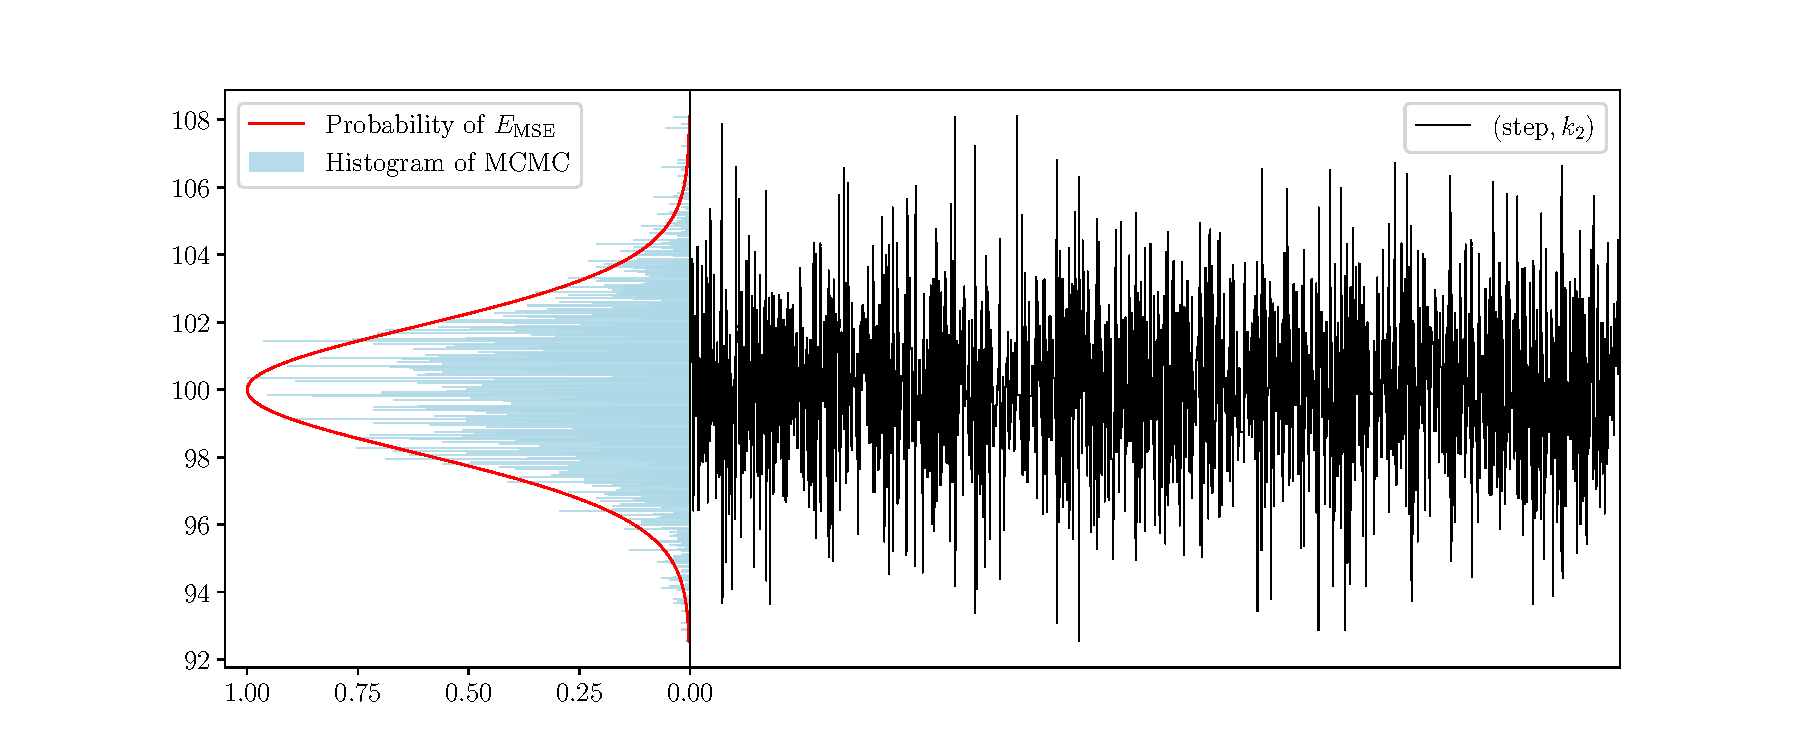
\includegraphics{/Users/yangchangmao/Documents/Coupled-Oscillators/MCMC-note/fig/MCMC-acc0.22080.pdf}

\end{document}




